%% Lee
%% In dissertation, change 
%    section* to chapter 
%    subsection* to section
%    subsubsection* to subsection

% #######################################################################################################################################
% >>>>>>>>>>>>>>>>>>>>>>>>>>> Results <<<<<<<<<<<<<<<<<<<<<<
\chapter{Results}
\label{sec:Results}
The objectives of this work was to design a system able to accelerate multiple disparate \acp{ann} in embedded systems.
\iffalse
This means systems that are not designed to process multiple requests of essentially the same operation.
\fi
Given that these systems cannot effectively utilize \ac{sram}, the main objective was to demonstrate a system that can operate efficiently using \ac{3ddram}.

The system decodes instructions, sends configuration to various functions, pre-fetchs and pipelines data.
This parallelism allows the system to constantly stream data whilst results from previous operations are being operated on.

To demonstrate such a system, this work targeted \ac{3dic} technology including \ac{3ddram}. This work proposes that if a system can be purely in \ac{3dic}, the system can take advantage of the benefits
of \ac{3dic} which includes reduced energy, area and high bandwidth.
In addition, this work proposes that given the system is \ac{3dic}, then a customized \ac{dram} would provide a significant bandwidth boost over typical implementations using standard DRAM.
\iffalse
To ensure the system was purely \ac{3dic}, the area of the system Manager and Processing Engine has to stay within the physical footprint of the \ac{3ddram}.
\fi

The target technology node was 28nm because its the technology node employed for some recent \acp{gpu} and other \acp{asic} such as \cite{jouppi2017datacenter}.
As a 28nm was not available to this team, the design was synthesized using an available 65nm technology node and then scaled to 28nm.

The primary control and datapaths of the system have been simulated in a system verilog environment. 
\iffalse
It has been synthesized using a 65nm technology node.
\fi
%The design has been coded . 
Initial synthesis timing closure at a frequency of \SI{500}{\mega\hertz} is complete.

\iffalse
As mention previously \eqref{eq:averageBandwidth}, to process multiple useful sized \acp{ann} requires a sustained bandwidth to the \ac{pe} of the order of ten's of \SI[per-mode=symbol]{}{\tera\bit\per\second}.
\fi

%%%%The approximate design targets are shown in Table \ref{tab:DesignTargets}.
%%%%
%%%%\begin{table}[h]
%%%%%  \captionsetup{justification=centering, skip=-5pt}
%%%%  \captionsetup{justification=centering, skip=3pt}
%%%%  \caption{Design targets}
%%%%  \label{tab:DesignTargets}
%%%%  \centering
%%%%%  \begin{center}
%%%%    % [lr] ~ left align col 0 and right align col 1
%%%%    % e.g. 4 columns could be lccr
%%%%    \begin{tabular}{lr}
%%%%      \toprule
%%%%      Parameter         & Target \\
%%%%      \midrule
%%%%      Frequency         & $>$\SI{700}{\MHz}   \\
%%%%      Power             & \SI{\approx 80}{\W}   \\
%%%%      Bandwidth         & \SI[per-mode=symbol]{\approx 64}{\tera\bit\per\second} \\
%%%%      Overall Die Area  & \SI{175}{\mm^2} \\
%%%%      \bottomrule
%%%%    \end{tabular}
%%%%%  \end{center}
%%%%\end{table}

Initial place and route for the Manager and \ac{pe} are shown in figure \ref{fig:Manager and PE Die layouts}. 
The area contribution of each block within the Manager and \ac{pe} can be seen in table \ref{tab:Area contribution}.
\begin{table}[h]
%  \captionsetup{justification=centering, skip=-5pt}
  \captionsetup{justification=centering, skip=3pt}
  \caption{Area Contribution}
  \vspace{3pt}
  \label{tab:Area contribution}
  \centering
    % [lr] ~ left align col 0 and right align col 1
    % e.g. 4 columns could be lccr
  \begin{subtable}{0.75\textwidth}
    \centering
    \begin{adjustbox}{width=0.75\textwidth}
      \begin{tabular}{ccc}
        \toprule
                            % \multicolumn{4}{c}{3D-DRAM Simulation-based estimates}   \\
                         &          &                                         \\  %\cline{1-1}
            Block        &Instances &Percentage                               \\  %\cline{1-1}
            Name         &          &Contribution                             \\  %\cline{1-1}
        \hline  % instead of \midrule %midrule doesnt overlap with column lines
  Memory Controller      & 1&\SI[per-mode=symbol]{15.0}{\percent}  \\ 
        NoC              & 1&\SI[per-mode=symbol]{ 7.1}{\percent}  \\
        Read Control     & 2&\SI[per-mode=symbol]{53.1}{\percent}  \\
        Write Control    & 1&\SI[per-mode=symbol]{ 7.4}{\percent}  \\
      Instruction Proc   & 1&\SI[per-mode=symbol]{ 1.6}{\percent}  \\
      Return Data Proc   & 1&\SI[per-mode=symbol]{ 1.6}{\percent}  \\
        Misc             & 1&\SI[per-mode=symbol]{14.2}{\percent}  \\
        \bottomrule
      \end{tabular}
    \end{adjustbox}
    \vspace{3pt}
    \captionsetup{justification=centering, skip=10pt}
    \caption{Manager}
    \label{tab:Manager Area Contribution}
  \end{subtable}
  \bigskip
  \begin{subtable}{0.75\textwidth}
    \centering
    \begin{adjustbox}{width=0.85\textwidth}
      \begin{tabular}{ccc}
        \toprule
                            % \multicolumn{4}{c}{3D-DRAM Simulation-based estimates}   \\
                         &          &                                          \\  %\cline{1-1}
            Block        &Instances & Percentage                               \\  %\cline{1-1}
            Name         &          & Contribution                             \\  %\cline{1-1}
        \hline  % instead of \midrule %midrule doesnt overlap with column lines
     Operation Decode    & 1&\SI[per-mode=symbol]{ 3.4}{\percent}  \\
   Return Data Control   & 1&\SI[per-mode=symbol]{ 1.5}{\percent}  \\
    SIMD Control         & 1&\SI[per-mode=symbol]{ 8.1}{\percent}  \\
        SIMD             & 1&\SI[per-mode=symbol]{19.3}{\percent}  \\
  Streaming Operations   &32&\SI[per-mode=symbol]{43.3}{\percent}  \\
  Streaming Op Control   & 1&\SI[per-mode=symbol]{ 2.1}{\percent}  \\
 Local Memory + Control\footnote{A small amount of scratchpad memory was provided between \acp{stop} and \ac{simd} but in practice could be much smaller. It is not used in any of the fanin tests.}  & 1&\SI[per-mode=symbol]{17.7}{\percent}  \\ 
        Misc             & 1&\SI[per-mode=symbol]{ 4.6}{\percent}  \\
        \bottomrule
      \end{tabular}
    \end{adjustbox}
    \vspace{3pt}
    \captionsetup{justification=centering, skip=10pt}
    \caption{PE}
    \label{tab:PE Area Contribution}
  \end{subtable}
  \end{table}


\iffalse
Although the design is yet to close timing, the 
\else
The
\fi
parasitics were extracted from these layouts and simulated against a group of operations. 
The operations simulated were based on the expected lower and upper limits of pre-synaptic fanin. 
These testcases were based on layers similar to CONV2 and FC-7 from \cite{krizhevsky2012imagenet} and represent a pre-synaptic fanin of 225 and 4000 respectively.
Additional testcases were employed representing pre-synaptic fanins of 294, 300, 500 and 1000. Both locally connected (CONV) and fully connected (FC) type fanins were tested.
The results showing sustained average bandwidth can be seen in table \ref{tab:Bandwidth Estimates}.

The simulation generated an activity file which was then used by the Synopsys\textregistered ~Primetime-PX\texttrademark ~power analysis tool to obtain power and bandwidth estimates.
The DRAM accesses were captured and DRAM energy dissipation calculated from \cite{tezzaron:diram4}. The power dissipated in the TSVs were estimated from \cite{liu2012compact}.
These estimates were used to estimate power dissipation for operating frequencies of \SI{500}{\mega\hertz} and \SI{700}{\mega\hertz}.
The estimated overall power along with per block contribution are shown in table \ref{tab:Simulation-based estimates}.

\begin{table}[h]
%  \captionsetup{justification=centering, skip=-5pt}
  \captionsetup{justification=centering, skip=3pt}
  \caption{Power Estimates}
  \vspace{3pt}
  \label{tab:Simulation-based estimates}
  \centering
    % [lr] ~ left align col 0 and right align col 1
    % e.g. 4 columns could be lccr
  \begin{subtable}{0.75\textwidth}
    \centering
    \begin{adjustbox}{width=0.85\textwidth}
      \begin{tabular}{cccc}
        \toprule
                            % \multicolumn{4}{c}{3D-DRAM Simulation-based estimates}   \\
                         &                       & Total    &                                          \\  %\cline{1-1}
            Technology   & Clock                 & Expected &                                          \\  %\cline{1-1}
                Node     & Frequency             &  Power   &  Testcase                                \\  %\cline{1-1}
        \hline  % instead of \midrule %midrule doesnt overlap with column lines
                   28nm  & \SI{500}{\mega\hertz} &   64W    &  CONV-294\iffalse \SI[per-mode=symbol]{\sim 70}{\percent} \fi \\ %\cline{2-2}
                   28nm  & \SI{700}{\mega\hertz} &   88W    &  CONV-294\iffalse \SI[per-mode=symbol]{\sim 70}{\percent} \fi \\ %\cline{2-2}
        \bottomrule
      \end{tabular}
    \end{adjustbox}
    \vspace{3pt}
    \captionsetup{justification=centering, skip=10pt}
    \caption{Power Dissipation}
    \label{tab:Power Dissipation}
  \end{subtable}
  \bigskip
  \begin{subtable}{0.75\textwidth}
    \centering
    \begin{adjustbox}{width=0.55\textwidth}
      \begin{tabular}{cc}
        \toprule
                            % \multicolumn{4}{c}{3D-DRAM Simulation-based estimates}   \\
                         &                                          \\  %\cline{1-1}
            Block        & Percentage                               \\  %\cline{1-1}
            Name         & Contribution                             \\  %\cline{1-1}
        \hline  % instead of \midrule %midrule doesnt overlap with column lines
                Manager  & \SI[per-mode=symbol]{66.6}{\percent}  \\ 
                     PE  & \SI[per-mode=symbol]{28.0}{\percent}  \\
                   DRAM  & \SI[per-mode=symbol]{ 2.5}{\percent}  \\
              DRAM TSVs  & \SI[per-mode=symbol]{ 1.8}{\percent}  \\
         Stack Bus TSVs  & \SI[per-mode=symbol]{ 1.2}{\percent}  \\
        \bottomrule
      \end{tabular}
    \end{adjustbox}
    \vspace{3pt}
    \captionsetup{justification=centering, skip=10pt}
    \caption{Power Contribution}
    \label{tab:Power Dissipation}
  \end{subtable}
  \end{table}

As bus efficiency is the main metric, table \ref{tab:Bandwidth Estimates} shows sustained average bandwidth over the fanin testcases.

\begin{table}[h]
%  \captionsetup{justification=centering, skip=-5pt}
  \captionsetup{justification=centering, skip=3pt}
  \caption{Fanin Bandwidth Tests}
  \vspace{3pt}
  \label{tab:Bandwidth Estimates}
  \centering
    \begin{adjustbox}{width=0.57\textwidth}
      \begin{tabular}{ccc}
        \toprule
                            % \multicolumn{4}{c}{3D-DRAM Simulation-based estimates}   \\
                                                       &                                         \multicolumn{2}{c}{Average Bandwidth}                      \\  %\cline{1-1}
                                                       &                                         \multicolumn{2}{c}{At Frequency}                                      \\  %\cline{1-1}
                   Test                                &        \SI{500}{\mega\hertz}                            & \SI{700}{\mega\hertz}                               \\  %\cline{1-1}
        \hline  % instead of \midrule %midrule doesnt ove        
                   CONV2 \cite{krizhevsky2012imagenet} &\ \SI[per-mode=symbol]{\sim 22}{\tera\bit\per\second}    & \SI[per-mode=symbol]{\sim 30}{\tera\bit\per\second} \\ %\cline{2-2}
                   CONV-294                            &\ \SI[per-mode=symbol]{\sim 23}{\tera\bit\per\second}    & \SI[per-mode=symbol]{\sim 31}{\tera\bit\per\second} \\ %\cline{2-2}
                   CONV-300                            &\ \SI[per-mode=symbol]{\sim 25}{\tera\bit\per\second}    & \SI[per-mode=symbol]{\sim 34}{\tera\bit\per\second} \\ %\cline{2-2}
                   CONV-500                            &\ \SI[per-mode=symbol]{\sim 26}{\tera\bit\per\second}    & \SI[per-mode=symbol]{\sim 38}{\tera\bit\per\second} \\ %\cline{2-2}
                   CONV-1000                           &\ \SI[per-mode=symbol]{\sim 30}{\tera\bit\per\second}    & \SI[per-mode=symbol]{\sim 41}{\tera\bit\per\second} \\ %\cline{2-2}
                   FC-350                              &\ \SI[per-mode=symbol]{\sim 26}{\tera\bit\per\second}    & \SI[per-mode=symbol]{\sim 36}{\tera\bit\per\second} \\ %\cline{2-2}
                   FC-500                              &\ \SI[per-mode=symbol]{\sim 27}{\tera\bit\per\second}    & \SI[per-mode=symbol]{\sim 38}{\tera\bit\per\second} \\ %\cline{2-2}
                   FC-1000                             &\ \SI[per-mode=symbol]{\sim 30}{\tera\bit\per\second}    & \SI[per-mode=symbol]{\sim 42}{\tera\bit\per\second} \\ %\cline{2-2}
                   FC-7 \cite{krizhevsky2012imagenet}  &\ \SI[per-mode=symbol]{\sim 31}{\tera\bit\per\second}    & \SI[per-mode=symbol]{\sim 43}{\tera\bit\per\second} \\ %\cline{2-2}
        \bottomrule
      \end{tabular}
    \end{adjustbox}
    \vspace{3pt}
  \end{table}

%%%%\begin{table}[h]
%%%%%  \captionsetup{justification=centering, skip=-5pt}
%%%%  \captionsetup{justification=centering, skip=3pt}
%%%%  \caption{Design targets}
%%%%  \label{tab:DesignTargets}
%%%%  \centering
%%%%%  \begin{center}
%%%%    % [lr] ~ left align col 0 and right align col 1
%%%%    % e.g. 4 columns could be lccr
%%%%    \begin{tabular}{lccccc}
%%%%          \toprule
%%%%                            %& \multicolumn{4}{c}{Technology}   \\
%%%%                            &       &       &  Usable    &          &  \\  %\cline{1-1}
%%%%                            &       &       &   DRAM     & Expected &  \\  %\cline{1-1}
%%%%                            & Tech  & Freq  & Bandwidth  &  Power   &  \\  %\cline{1-1}
%%%%          \hline  % instead of \midrule %midrule doesnt overlap with column lines
%%%%                  3D-System & 28    & \SI{700}{\mega\hertz}      &       \SI[per-mode=symbol]{\sim 64}{\tera\bit\per\second}   &  73W   &  \\ %\cline{2-2}
%%%%                  NVidia    & 28    &       &  $\ll$\SI[per-mode=symbol]{1.28}{\tera\bit\per\second} &  100W  &  \\
%%%%                  TPU       & 28    &       &  $<$  \SI[per-mode=symbol]{224}{\giga\bit\per\second}  &  40W   &  \\
%%%%          \bottomrule
%%%%    \end{tabular}
%%%%%  \end{center}
%%%%\end{table}


\begin{figure}[h]
\centering
\begin{subfigure}{.5\textwidth}
  \centering
  \centerline{
    \mbox{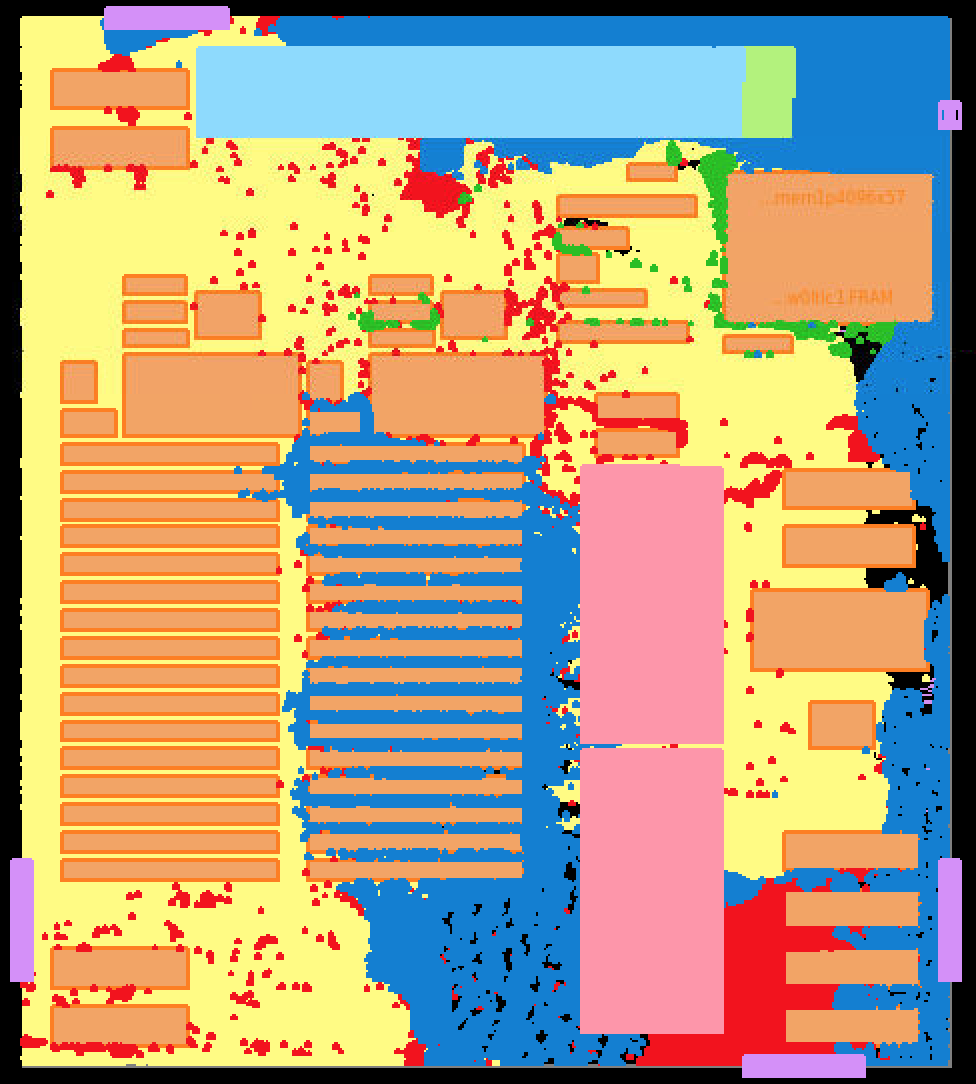
\includegraphics[width=1\linewidth]{ManagerLayout.png}}
  }
  \captionsetup{justification=centering, width=.8\linewidth}
  \caption{Manager}
  %\vspace{40pt}
  \label{fig:managerLayout}
\end{subfigure}%

\bigskip

\begin{subfigure}{.5\textwidth}
  \centering
  \centerline{
    \mbox{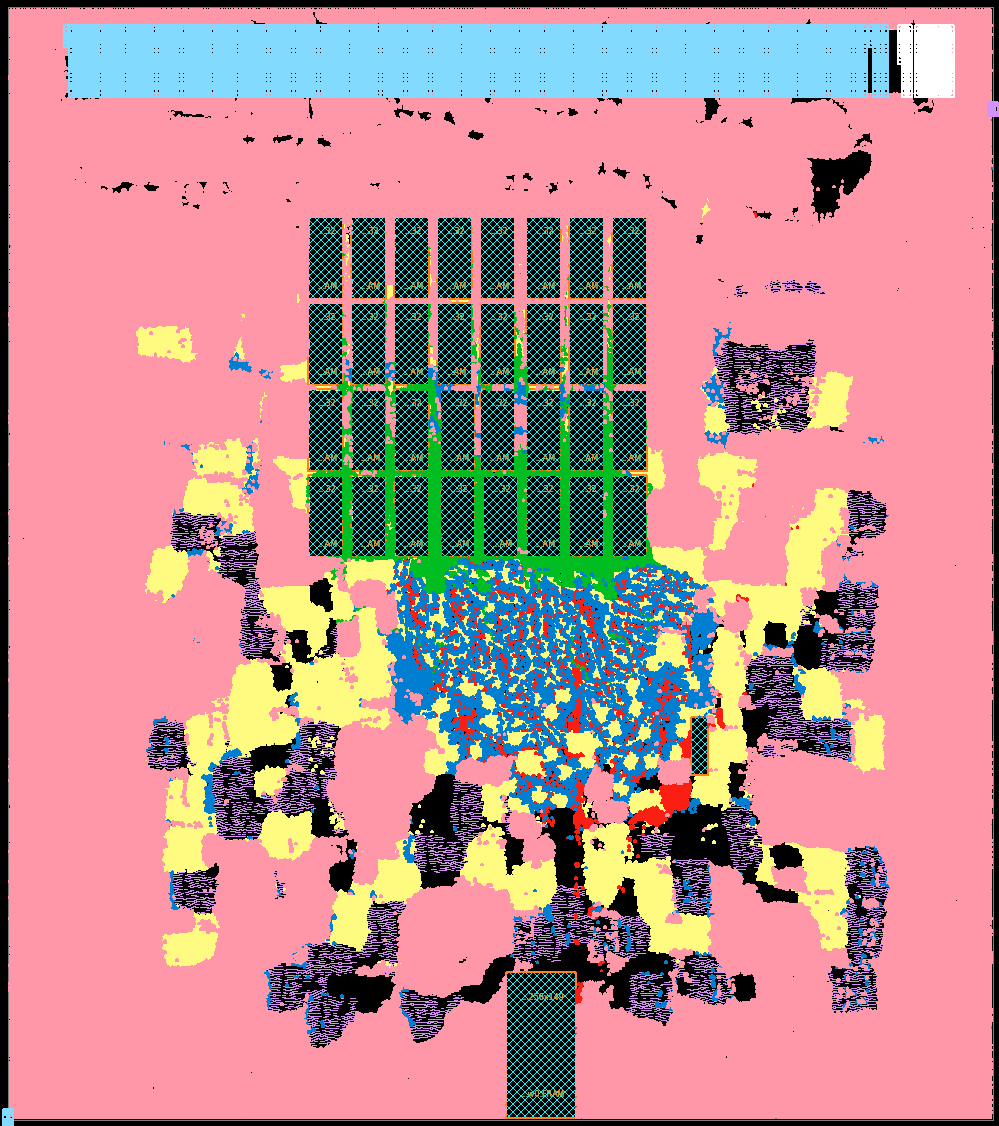
\includegraphics[width=1\linewidth]{PElayout.png}}
  }
  \captionsetup{justification=centering, width=.8\linewidth}
  \caption{PE}
  \label{fig:peLayout}
\end{subfigure}
\captionsetup{justification=centering, width=.9\linewidth}
\caption{Manager and PE Die layouts}
\label{fig:Manager and PE Die layouts}
\end{figure}



